\section{CMB Analyse}

% TODO Acronyms
Die Analyse des CMB Leistungsspektrums wird mit Hilfe der in einer 
Semesterarbeit entwickelte SHCL Library (zu finden auf Github unter 
\url{https://github.com/Darnor/SHCL}) durchgeführt.

\subsection{Was sind unsere Daten}
Als Datengrundlage wird erst das öffentlich verfügbare CMB Bild in 
Rektangularprojektion \ref{bib:cmb_public_equirectangular} verwendet.

\begin{figure}
	\centering
	\includegraphics[width=\linewidth]{cmb/images/CMB_Planck_E.jpg}
	\caption{Das generierte Bild des CMB in Rektangularprojektion der ESA 
	Planck mission, welches die Datengrundlage für die Analyse liefert.}
	\label{fig:cmb-rectangular}
\end{figure}
% TODO: Image CMB (rectangular)
% TODO: Aufzeugung funktion der conversiation RBG -> "Kelvin"

\subsection{Das Leistungsspektrum}

% TODO: Erklärung C_l
% TODO: diff cosmic variance \Delta C_l und C_l

\subsection{Spärische harmonische Koeffizienten}
% TODO: c_l^m erklärung
% TODO: Problemstellung bei berechnung rauschen -> grosse zahl -> lösung

\subsection{Resultate}

\begin{figure}
	\centering
	
\includegraphics[width=\linewidth]{cmb/images/color-strip-full.png}
	\caption{Farbverlauf der für die Codierung des CMB Bildes der ESA Planck 
	Mission verwendet wurde.}
	\label{fig:color-strip-orig}
\end{figure}

\begin{figure}
	\centering
	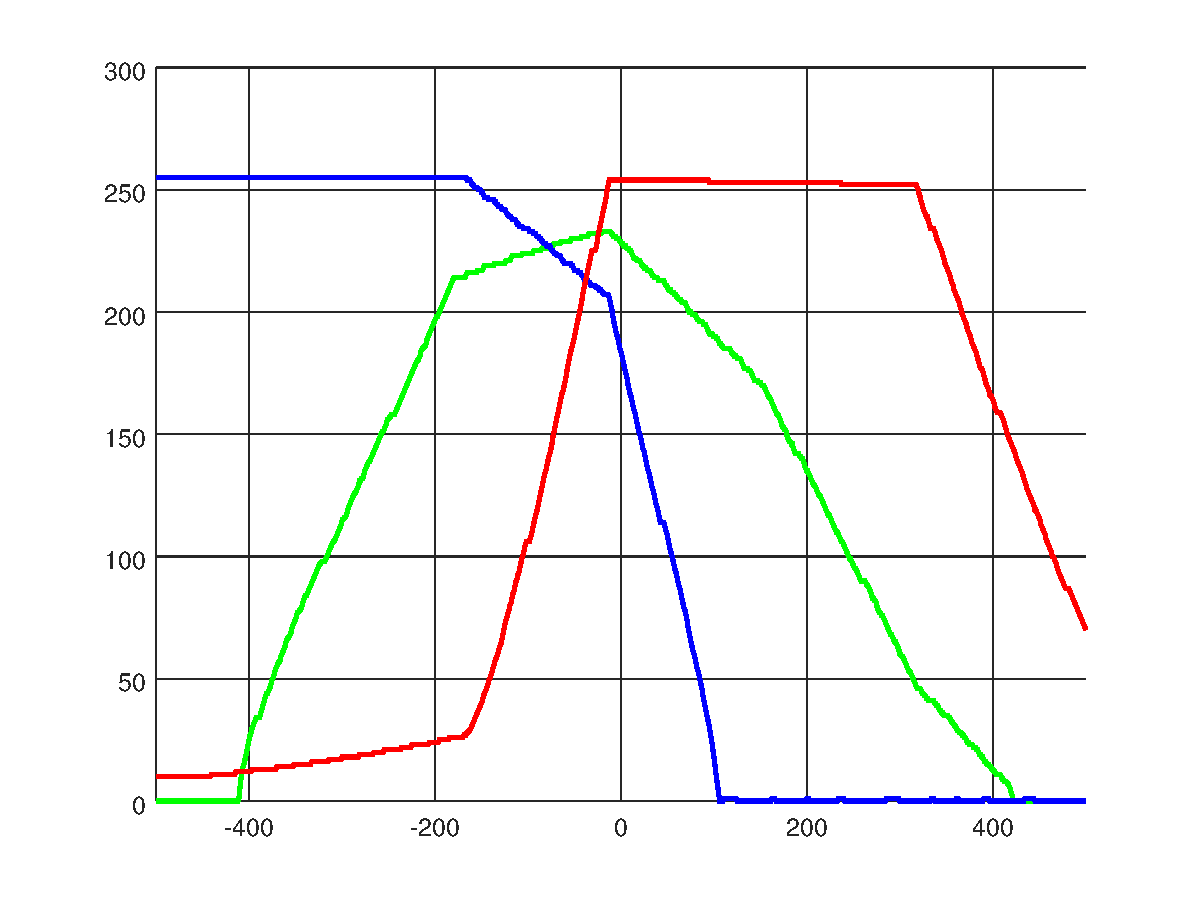
\includegraphics[width=\linewidth]{cmb/converter/rgb-graph.pdf}
	\caption{RGB Profil des in Abbildung~\ref{fig:color-strip-orig} 
	verwendeten Farbverlaufs.}
	\label{fig:color-strip-orig-rgb}
\end{figure}

Abbildung \ref{fig:cmb-power-spec-2000} zeigt, was wir mit unseren Berechnungen 
ein ähnliches Bild wie erwartet bekommen. Natürlich ist das ganze nicht 
perfekt, so stimmt die $l(l+1)C_l/2\pi$ Skala um rund einen Faktor 10 nicht mit 
dem erwarteten überein. Das alles macht deutlich, dass unsere Umwandlung der 
RGB Werte in Kelvin nicht ganz korrekt ist.

\begin{figure}
	\centering
	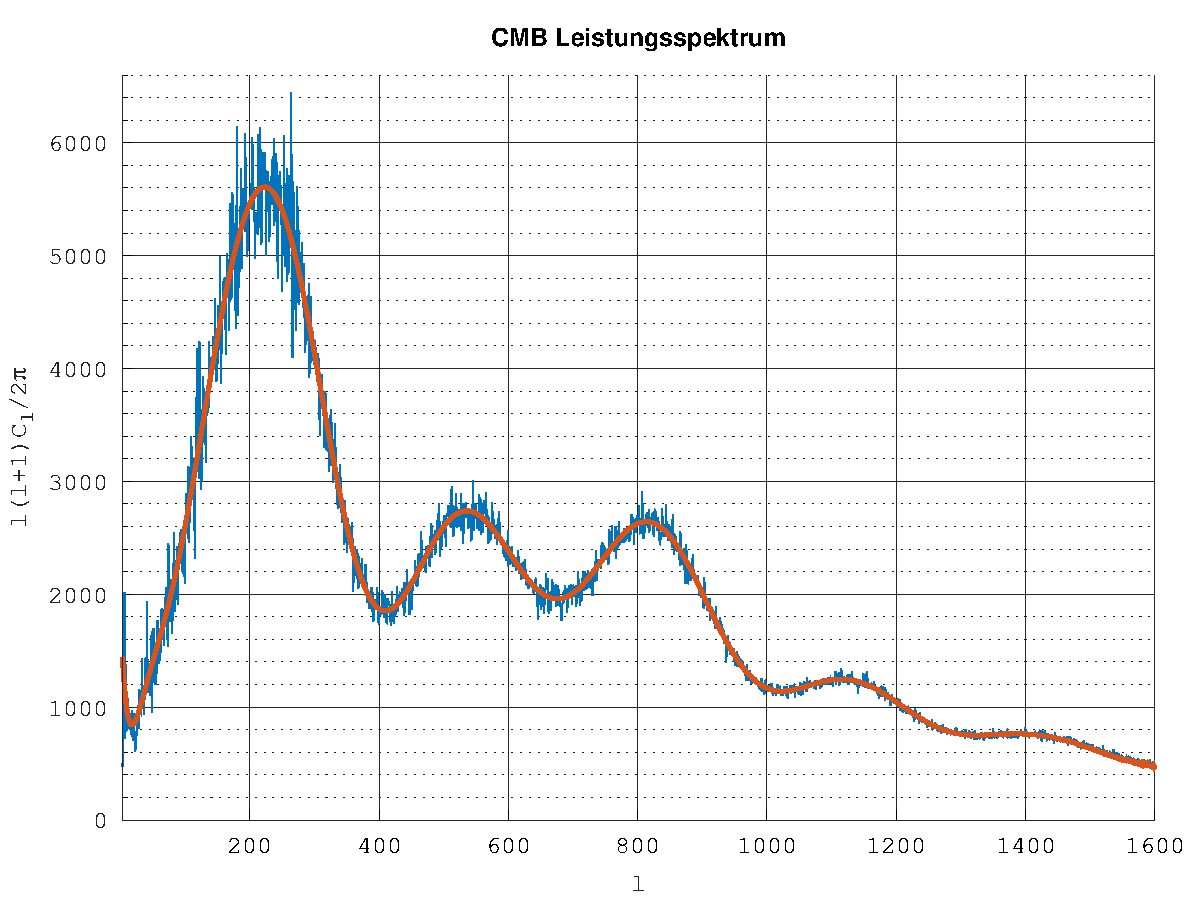
\includegraphics[width=\linewidth]{cmb/data/4k1800-500.pdf}
	\caption{Leistungsspektrum berechnet bis zu $l = 1600$. Grundlage für die 
		Berechnung sind die 4k Bilder der ESA Planck Mission.}
	\label{fig:cmb-power-spec-1600}
\end{figure}

\begin{figure}
	\centering
	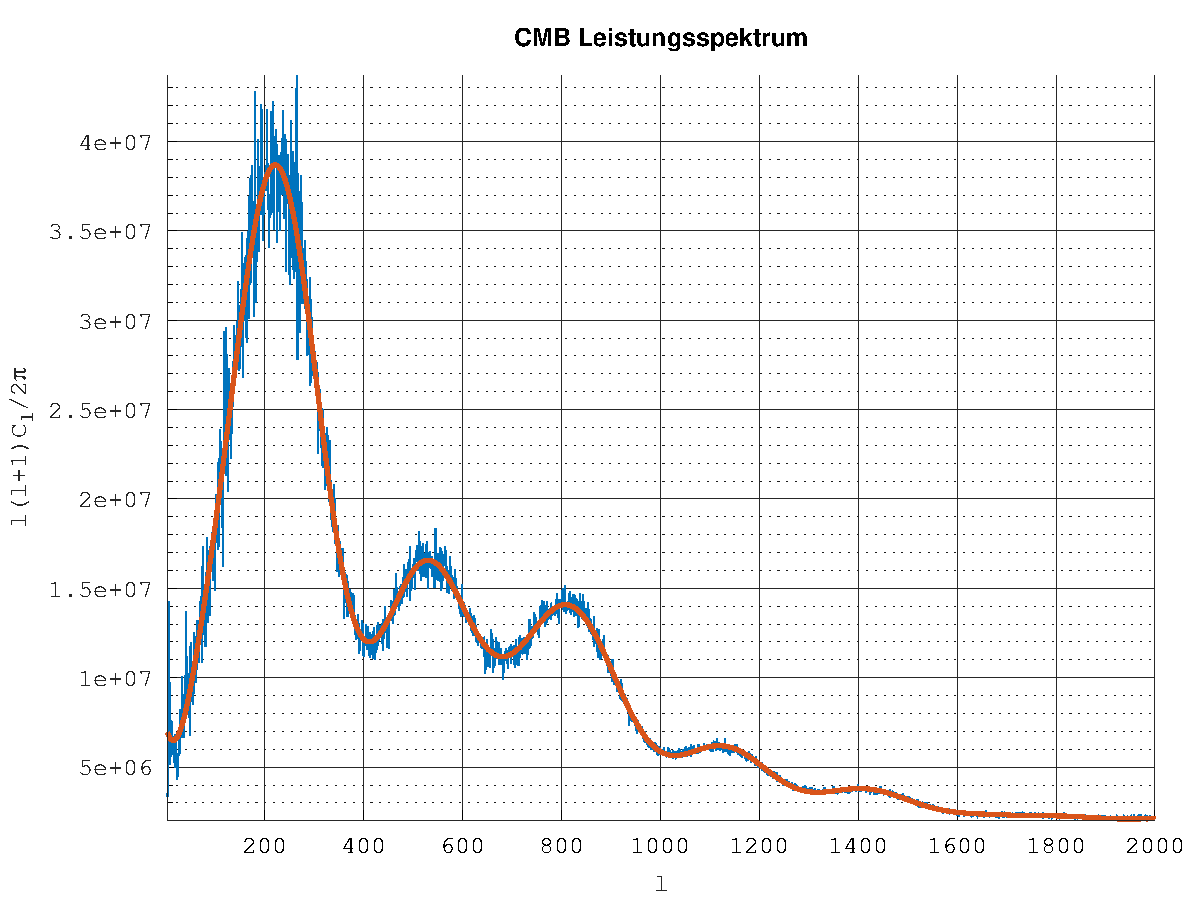
\includegraphics[width=\linewidth]{cmb/data/12k2500-500.pdf}
	\caption{Leistungsspektrum berechnet bis zu $l = 2000$. Grundlage für die 
	Berechnung sind die 12k Bilder der ESA Planck Mission.}
	\label{fig:cmb-power-spec-2000}
\end{figure}

% TODO: Resultate zeigen